%----------------------------------------------------------------------------
%\Aref{sect:chapter_test}. fejezetben több valós hálózatot vizsgálok meg az addigra meghatározott saját policy-k segítségével, és megvizsgálom a keverék policy pontosságát, azaz azt, hogy mennyire térnének el a valós hálózatbeli utak a jelenlegitől akkor, ha az általam ismertetett policy-kel határoznánk meg azokat.
%----------------------------------------------------------------------------
\chapter{Repülési hálózat vizsgálata}\label{sect:chapter_test}
%----------------------------------------------------------------------------

Az \href{http://openflights.org/}{openflights.org} oldalon elérhető repülési adatbázis feldolgozása és szimulációs elemzése az egyik olyan feladat, amit a következő félév végéig fogok elvégezni. Az oldal lehetőséget biztosít interaktív keresésre, regisztráció után pedig statisztikákat készíthetünk saját utazásainkról. Emellett elérhető a teljes adatbázisa is, amit többek között hivatalos forrásokból, illetve a felhasználóktól gyűjt.

  %----------------------------------------------------------------------------
  \section{Az adatok}
  %----------------------------------------------------------------------------

  Az openflights-on elérhető adatbázis világszerte mindenhonnan gyűjt és tárol reptéri, repülési társasági és repülési út adatokat. Közel 8000 reptér, 6000 társaság és 60000 repülési út érhető el. Részletes adatok \aref{tab:table_repterek},~\aref{tab:table_repulesitarsasagok}, és a \aref{tab:table_repulesiutvonalak} táblázatokban.

    %----------------------------------------------------------------------------
    \subsection{Repterek}
    %----------------------------------------------------------------------------

    \begin{figure}[!ht]
      \centering
      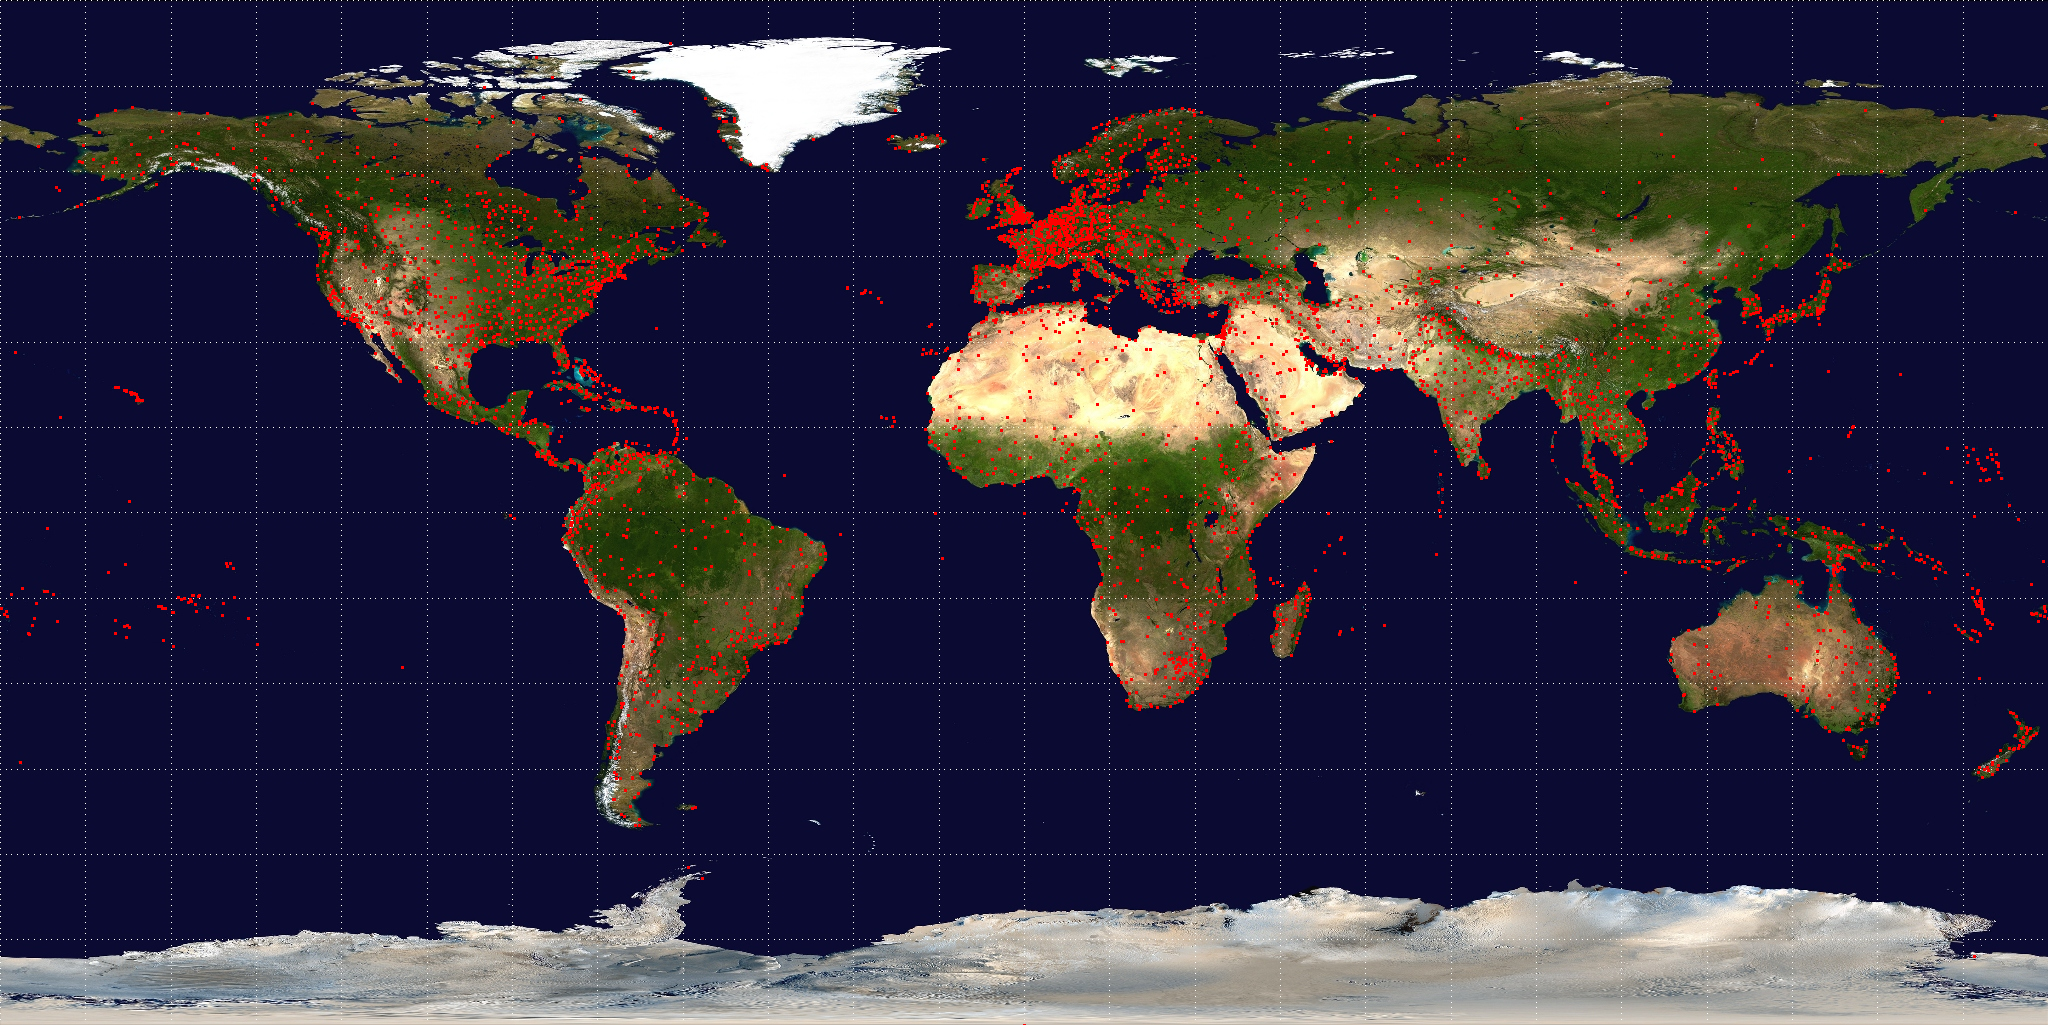
\includegraphics[width=150mm,keepaspectratio=true]{./figures/airports-2048.png}
      % airports-2048.png: 2048x1025 pixel, 96dpi, 54.18x27.12 cm
      
      \caption{Az OpenFights adatbázisában szereplő repterek.}
      \label{fig:figure_repterek}
    \end{figure}

    A rendszer tárolja a repterek \emph{nevét}; a \emph{várost}, ahol található; a \emph{szélességi}- és \emph{hosszúsági fokokat}, illetve a \emph{tengerszint feletti magasságot}. Emellett elérhető a repülési hatóságok által használt 3 karakter hosszú \emph{IATA\footnote{International Air Transport Association: Nemzetközi Légi Szállítási Szövetség}/FAA\footnote{Federal Aviation Administration: Szövetségi Légügyi Hivatal (USA)} azonosító} is és az OpenFlights által használt decimális \emph{azonosító} is. A legutolsó, 2014 januári frissítéskor az OpenFlights adatbázisa 7733 repteret tartalmazott világszerte, ezt mutatja \aref{fig:figure_repterek} ábra.

    \begin{table}[ht]
      \footnotesize
      \centering
      \caption{Az OpenFlights adatbázisában elérhető reptéri adatok.}
      \begin{tabular}{ | l | l |}
      \hline
      Attribútum & Leírás \\ \hline
      Airport ID & Egyedi OpenFlights azonosító.\\
      Name & A reptér neve.\\
      City & Az a város, amit a reptér ,,kiszolgál''.\\
      Country & Az ország vagy terület neve, ahol reptér található.\\
      IATA/FAA & 3 betűs FAA kód az USA-beli reptereknek vagy 3 betűs IATA kód, minden más esetben.\\
      ICAO\footnote{International Civil Aviation Organization: Nemzetközi Polgári Repülési Szervezet} & 4 betűs ICAO kód.\\
      Latitude & A reptér szélességi foka: decimális szám (fokban mérve), általában 6 szignifikáns jegyig.\\
      & A Déli féltekén negatív, az Északin pozitív.\\
      Longitude & A reptér hosszúsági foka: decimális szám (fokban mérve), általában 6 szignifikáns jegyig.\\
      & A Nyugati féltekén negatív, a Keletin pozitív.\\
      Altitude & A tengerszint feletti magasság, lábban mérve (1 láb $\sim$ 0.30 méter).\\
      \hline
      \end{tabular}
      \label{tab:table_repterek}
    \end{table}\newpage

    %----------------------------------------------------------------------------
    \subsection{Repülési útvonalak}
    %----------------------------------------------------------------------------

    \begin{figure}[!ht]
      \centering
      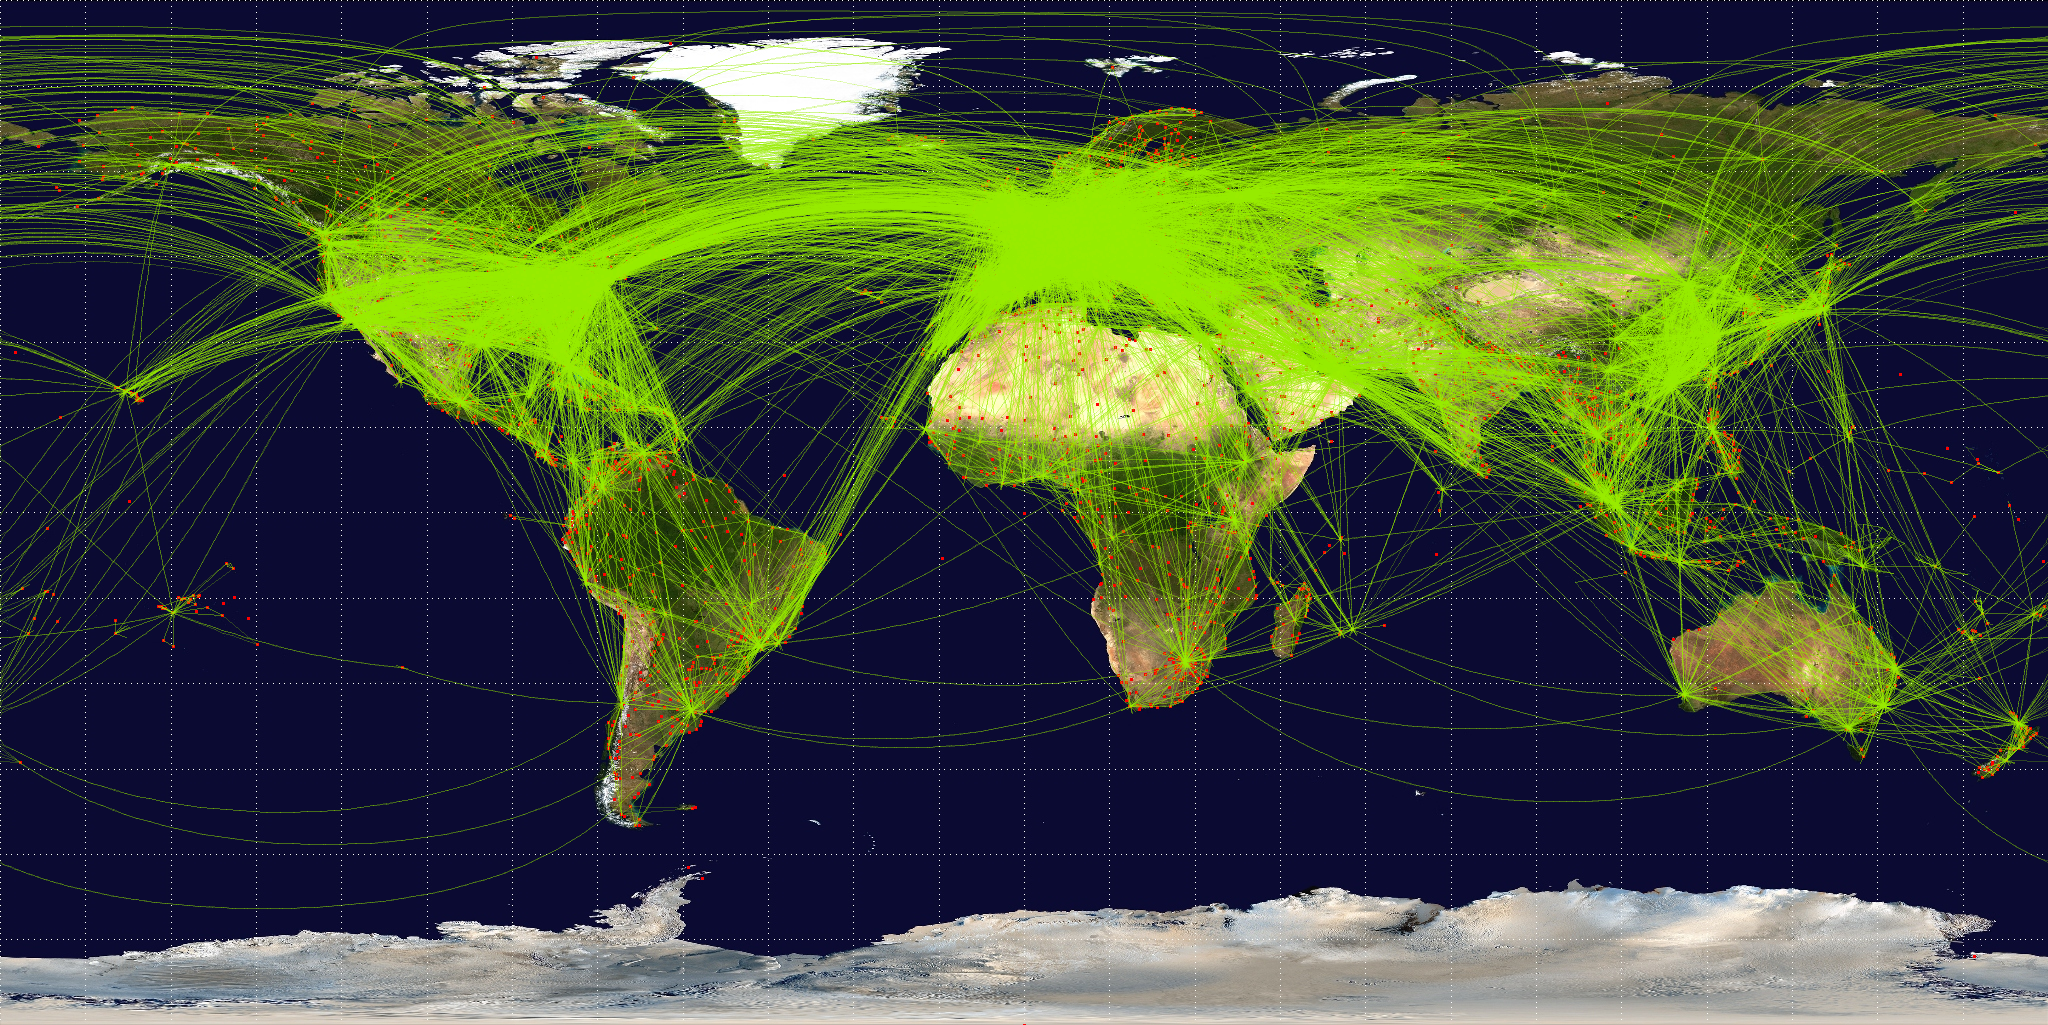
\includegraphics[width=150mm,keepaspectratio=true]{./figures/routes-2048.png}
      % routes-2048.png: 2048x1025 pixel, 96dpi, 54.18x27.12 cm
      
      \caption{Az OpenFights adatbázisában szereplő repülési útvonalak.}
      \label{fig:figure_repulesiutvonalak}
    \end{figure}

    A repülési útvonalak leírása öt attribútumot tartalmaz: az \emph{üzemeltető repülési társaság} (név és OpenFlights azonosító); a \emph{forrás reptér}; a \emph{cél reptér}. Emellett feljegyzik a \emph{megállások számát}\footnote{Az összesen 59637 bejegyzésből 6 esetében van 1 megállás és 1 esetben 2 megállás.}, illetve az ebben a viszonylatban használt \emph{repülőgép típusokat}. Ha két reptér között oda-vissza is van járat, akkor ez az adathalmazban két bejegyzésként jelenik meg. Jelenleg az OpenFlights adatbázisa 59637 útvonalat tartalmazott 3285 reptér és 531 társaság\footnote{Ugyan a légitársaság és reptér adatbázisokban ennél jelentősen több bejegyzés van, ám azok között vannak nem aktív társaságok, illetve bezárt repterek.} között világszerte, ahogy \aref{fig:figure_repulesiutvonalak} ábra is mutatja.

    \begin{table}[ht]
      \footnotesize
      \centering
      \caption{Az OpenFlights adatbázisában elérhető adatok a repülési útvonalakról.}
      \begin{tabular}{ | l | l |}
      \hline
      Attribútum & Leírás \\ \hline
      Airline & Az üzemeltető társaság 2 betűs (IATA) vagy 3 betűs (ICAO) kódja.\\
      Airline ID & Az üzemeltető társaság egyedi OpenFlights azonosítója.\\
      Source airport & A forrás reptér 3 betűs (IATA) vagy 4 betűs (ICAO) kódja.\\
      Source airport ID & A forrás reptér egyedi OpenFlights azonosítója.\\
      Destination airport & A cél reptér 3 betűs (IATA) vagy 4 betűs (ICAO) kódja.\\
      Destination airport ID & A cél reptér egyedi OpenFlights azonosítója.\\
      Codeshare & Igaz, ha a járat ,,codeshare'', azaz nem utasszállító járat, különben üres.\\
      Stops & A megállások szám (nem az átszállásokat jelenti, a ,,0'' jelenti a direkt járatot).\\
      Equipment & A viszonylatban használt repülőgép típusok 3 betűs kódjai.\\
      \hline
      \end{tabular}
      \label{tab:table_repulesiutvonalak}
    \end{table}\newpage

    %----------------------------------------------------------------------------
    \subsection{Repülési társaságok}
    %----------------------------------------------------------------------------

    A repülési társaságokról tárolt adatok többek között tartalmazzák a hivatalos \emph{IATA azonosítót}; a cég \emph{nevét}; az \emph{országot}, ahol be van jegyezve; illetve, hogy \emph{aktív-e} még a társaság. Emellett természetesen itt is definiáltak egy saját (OpenFlights) \emph{azonosítót}.

    \begin{table}[ht]
      \footnotesize
      \centering
      \caption{Az OpenFlights adatbázisában elérhető adatok a repülési társaságokról.}
      \begin{tabular}{ | l | l |}
      \hline
      Attribútum & Leírás \\ \hline
      Airport ID & Egyedi OpenFlights azonosító.\\
      Name & A társaság neve.\\
      Alias & A társaság egyéb megnevezése.\\
      IATA & 2 betűs IATA kód.\\
      ICAO & 3 betűs ICAO kód.\\
      Callsign & A társaság hívójele.\\
      Country & Az ország vagy terület neve, ahol a társaság be van jegyezve.\\
      Active & Igaz, ha a társaság jelenleg is, vagy nemrég még működött (nem megbízható).\\
      \hline
      \end{tabular}
      \label{tab:table_repulesitarsasagok}
    \end{table}

  %----------------------------------------------------------------------------
  \section{A szimuláció}
  %----------------------------------------------------------------------------
    %----------------------------------------------------------------------------
    \subsection{Az adatok előfeldolgozása}
    %----------------------------------------------------------------------------

    A modellezendő hálózat első megközelítésben az összes csomópontból alkotott $K_{7733}$ teljes gráf. Ez természetesen feleslegesen nagy vizsgálandó hálózatot jelentene ($7733 \choose 2$ = 29.895.778 élű gráf.), emellett az olyan, leíró jellegű jellemzők, mint a valódi hálózat átmérője, vagy pont- és él-összefüggőségei elvesznének. Lévén a repülési hálózat skálafüggetlen - sok olyan csomópont van, ahova csak adott, kis számú, közeli csomópontokból indulnak járatok, így nem érdemes összekötni távoli csomópontokkal. Ezenkívül a repülésnél vannak olyan szempontok, amelyeket az útvonalválasztásnál figyelembe vesznek, ám én ezek pontos információk hiányában nem tudom kezelni - pl. csak adott hosszúságú utat tehet meg egy adott típusú repülőgép az üzemanyagtartálya méretétől függően.

    %----------------------------------------------------------------------------
    \subsection{A szimuláció megtervezése}
    %----------------------------------------------------------------------------

    A fentiek miatt a szimulált hálózatot a következőképpen határozom meg: pontjai a repterek, élei pedig, az adatbázisban szereplő össze, megállás nélküli repülőút. Így magától értetődően csak olyan élek lesznek a szimulációban, amelyek ,,átrepülhetők'', hiszen volt már, hogy átrepülték. Emellett pedig ez a hálózat hűen tükrözi a valóságot, hiszen feltehetjük, hogy csak azon élek nincsenek behúzva, amelyeket repüléstechnikai okokból nem is lehet, különben valaki, valamikor már repült volna azon az úton.\\

    Az útvonalválasztást a 10 legjelentősebb légitársaság alapján szimulálom, mert a 10 legtöbb járatot üzemeltető társaság az utak 24\%-át adják. A policy vezérelt útvonalválasztást az összes olyan pontpár között lefuttatom, amely ezen 10 társaság célpontja.

    % 5209 (2417), 4296 (2186), 2009 (1520), 24 (1513), 5265 (1381), 751 (1227), 1767 (1152), 1758 (1097), 4547 (1018), 3320 (931), 


    %----------------------------------------------------------------------------
    \subsection{A vizsgálandó metrikák, az élek súlyozása}
    %----------------------------------------------------------------------------

    A fejezet elején említett két megközelítést fogom alkalmazni, azaz a pont-pont kapcsolatokat is összehasonlítom és a globális hálózat mutatóit is. Az élek súlya annak megfelelően változik, hogy milyen policy algebráját szimulálom. Emellett a repterek GPS koordinátái alapján meghatározom az összekötött repterek fizikai távolságát. Mivel a légtérben nincsen torlódás az út szélességének definiálásának nincs értelme.\\

    A globális hálózati metrikák közül a fokszámeloszlást fogom vizsgálni, illetve a hálózat átmérőjét és a pont- és él-összefüggőségét. A fokszámeloszlás és az átmérő összehasonlításra azért van szükség, mert ezek alapvető karakterisztikáját adják a hálózatnak. A pont- és él-összefüggőséget pedig azért, mert ezek lehetnek olyan tényezők, amik a repülőtársaságok útvonalválasztása mögött meghúzódhatnak.
    
  %----------------------------------------------------------------------------
  \section{Az eredmények}
  %----------------------------------------------------------------------------

  %----------------------------------------------------------------------------
  \section{Összefoglaló}
  %----------------------------------------------------------------------------
